\documentclass{ieeeaccess}
\usepackage{cite}
\usepackage{amsmath,amssymb,amsfonts}
\usepackage{graphicx}
\usepackage{textcomp}
\usepackage[hyphens]{url}
\usepackage{bm}
\usepackage{amsthm}
\usepackage{float}
\usepackage{booktabs}
\usepackage[font=small,labelfont=bf]{caption}
\usepackage{placeins}


\renewcommand{\thetable}{\Roman{table}}

\graphicspath{{../figures/}}

% Generated table rows (scripts/make_exp04_tables.py). The TeX primitive is
% used because LaTeX's \input is not expandable inside a booktabs tabular.
% Long repository URL: allow breaks after any character.
\makeatletter\g@addto@macro{\UrlBreaks}{\do\a\do\b\do\c\do\d\do\e\do\f\do\g\do\h\do\i\do\j\do\k\do\l\do\m\do\n\do\o\do\p\do\q\do\r\do\s\do\t\do\u\do\v\do\w\do\x\do\y\do\z\do\A\do\C\do\D\do\E\do\F\do\I\do\M\do\S\do\V}\makeatother
\makeatletter\newcommand{\tabinput}[1]{\@@input #1 }\makeatother

\theoremstyle{definition}
\newtheorem{definition}{Definition}
\newtheorem{remark}{Remark}
\theoremstyle{plain}
\newtheorem{proposition}{Proposition}

\floatstyle{ruled}
\newfloat{algorithm}{tbp}{loa}
\floatname{algorithm}{Algorithm}
\newcounter{algstep}
\newenvironment{algsteps}{%
  \footnotesize
  \setcounter{algstep}{0}%
  \begin{list}{\textbf{\thealgstep:}}{%
    \usecounter{algstep}%
    \setlength{\labelwidth}{14pt}%
    \setlength{\labelsep}{4pt}%
    \setlength{\leftmargin}{20pt}%
    \setlength{\rightmargin}{0pt}%
    \setlength{\itemsep}{1pt}%
    \setlength{\parsep}{0pt}%
    \setlength{\topsep}{3pt}%
  }%
}{\end{list}}
\newcommand{\algind}[1]{\hspace*{#1.1em}}
\newcommand{\algkw}[1]{\textbf{#1}}
\newcommand{\algcomment}[1]{\textit{$\triangleright$~#1}}
\makeatletter
\AtBeginDocument{\DeclareMathVersion{bold}
\SetSymbolFont{operators}{bold}{T1}{times}{b}{n}
\SetSymbolFont{NewLetters}{bold}{T1}{times}{b}{it}
\SetMathAlphabet{\mathrm}{bold}{T1}{times}{b}{n}
\SetMathAlphabet{\mathit}{bold}{T1}{times}{b}{it}
\SetMathAlphabet{\mathbf}{bold}{T1}{times}{b}{n}
\SetMathAlphabet{\mathtt}{bold}{OT1}{pcr}{b}{n}
\SetSymbolFont{symbols}{bold}{OMS}{cmsy}{b}{n}
\renewcommand\boldmath{\@nomath\boldmath\mathversion{bold}}}
\makeatother

\def\BibTeX{{\rm B\kern-.05em{\sc i\kern-.025em b}\kern-.08em
    T\kern-.1667em\lower.7ex\hbox{E}\kern-.125emX}}

\AtBeginDocument{\renewcommand{\ttdefault}{lmtt}}

\makeatletter
\newcommand{\needspace}[1]{%
  \begingroup
    \setlength\dimen@{#1}%
    \vskip\z@\@plus\dimen@
    \penalty -100\vskip\z@\@plus -\dimen@
    \vskip\dimen@
    \penalty 9999%
    \vskip -\dimen@
    \vskip\z@skip
  \endgroup
}
\makeatother

\makeatletter
\renewenvironment{IEEEbiographynophoto}[1]{%
  \normalfont\@IEEEcompsoconly{\sffamily}\footnotesize\interlinepenalty500%
  \vskip 1\baselineskip minus 0\baselineskip%
  \parskip=0pt\par%
  \noindent\textbf{#1\ }\@IEEEgobbleleadPARNLSP}{\relax\par\normalfont}
\makeatother

\begin{document}
\history{Date of publication xxxx 00, 0000, date of current version xxxx 00, 0000.}
% Volume and year assigned by IEEE after acceptance; placeholder year for draft.
\year{2026}
% Volume is assigned by IEEE on acceptance; placeholder until then.
\vol{XX}
\doi{10.1109/ACCESS.XXXX.DOI}

\title{Lineage and Release Timing in Correlated Errors of Open-Weight Language Models: A Pre-Registered Pair-Level Study}

\author{\uppercase{Sudharsan S}\authorrefmark{1},
\uppercase{S. Kanaga Suba Raja}\authorrefmark{1,2},
\uppercase{Shree Harish V}\authorrefmark{1,3},
\uppercase{Chin-Shiuh Shieh}\authorrefmark{2},
\uppercase{Mong-Fong Horng}\authorrefmark{2},
\uppercase{Lavanya R}\authorrefmark{1}}

\address[1]{Department of Computer Science and Engineering, SRM Institute of
Science and Technology, Tiruchirappalli 620101, India}

\address[2]{Research Institute of IoT Cybersecurity, Department of Electrical
Engineering, National Kaohsiung University of Science and Technology,
Kaohsiung 824, Taiwan, ROC}

\address[3]{Department of Computer Science and Engineering (Big Data Analytics),
SRM Institute of Science and Technology,
Tiruchirappalli 620101, India}

\markboth
{Sudharsan \emph{et al.}: Lineage and Release Timing in Correlated LLM Errors}
{Sudharsan \emph{et al.}: Lineage and Release Timing in Correlated LLM Errors}

\corresp{Corresponding author: S. Kanaga Suba Raja (e-mail: kanagass@srmist.edu.in).}

\begin{abstract}
Ensembles and review pipelines built from several open-weight language models assume that their members err somewhat independently. When two models share an ancestor, or were released at the same time, that assumption may fail. We ask which of the two is associated with models choosing the \emph{same wrong answer}. We first show why the question cannot be answered by decomposing per-model accuracy into family and release-era variance components: in a precision analysis of the fitted random-effects model, every design we examined with five to seven model families and at most fourteen release quarters had a worst-case root-mean-square error (RMSE) of at least 0.18 for one of the two variance shares; more models per family helped only up to that point. We therefore move to a pair-level design. Using item-level predictions from the Open LLM Leaderboard (MMLU, 14{,}042 items), validated item by item against the leaderboard's stored correctness for 977 models in two overlapping populations, we resolve each model's lineage root from Hugging Face \texttt{base\_model} declarations and relate pairwise agreement on wrong answers to shared lineage and to the gap between upload months. The analysis, sample rules and a simulation-based power gate were fixed before any pairwise outcome was computed; three dated amendments are disclosed, one of which added two sensitivity analyses after per-model accuracies were seen. A post-hoc high-replication audit shows that the gate meets its null and power criteria but narrowly misses its cross-leakage criterion at the largest simulated release-time effect (10.8\% against a 10\% limit). In the pre-registered primary analysis (590 models, 173{,}755 pairs), sharing a lineage root is associated with a 13.3 percentage-point higher probability of choosing the same wrong option when both models err (95\% CI 11.8--14.8; delete-one-root jackknife CI 10.8--15.8), against a mean of 42.3\%. The estimate is 11.7--13.4 points across all twelve pre-registered analyses and stays between 10.2 and 14.2 points under root-level inference, alternative weighting, a position-adjusted outcome and exploratory size controls. Item-difficulty-aware null models absorb almost all of the average agreement but leave the lineage contrast unchanged. Unadjusted, same-month pairs agree 8.7 points more than pairs released a year or more apart, but this gradient is fully accounted for by the similarity of the two models' accuracies; net of accuracy, the association of release-month proximity with the choice of wrong option is not stable in sign or magnitude across specifications: the same-month coefficient is $+0.004$ (CI $-0.003$ to $+0.011$) in the primary analysis, small and positive under some weightings, and negative ($-0.015$, CI $-0.027$ to $-0.002$) among models scoring at least 30\%; for which items fail together, a small positive association appears in the full samples but not among models above 30\%. The associations are observational and describe a population dominated by community fine-tunes; they do not separate the pretraining era of foundation models from their lineage.
\end{abstract}

\begin{keywords}
Large language models, correlated errors, model lineage, ensembles, dyadic regression, pre-registration, Open LLM Leaderboard
\end{keywords}

\titlepgskip=-21pt

\maketitle

\section{Introduction}
\label{sec:introduction}

\PARstart{W}{hen} several public language models are asked the same hard question, they often fail together, and often in the same way. Kim~\textit{et al.}~\cite{kim2025} document this across hundreds of open and hosted models: when two models are both wrong, they choose the same wrong option far more often than chance. For anyone who combines models---a majority vote, a routing scheme, or a review step that escalates only when models disagree---this matters directly. Agreement between members is informative only if their errors are not shared~\cite{dietterich2000,kuncheva2003}.

Two explanations for shared errors compete. \emph{Lineage}: a model fine-tuned from another inherits its parameters and therefore, plausibly, its blind spots. \emph{Era}: models built at the same time draw on the same data, recipes and fashions and may acquire the same mistakes without any shared ancestry. The two are entangled, because descendants are always released after their ancestors. Which one dominates has a practical consequence: if lineage dominates, combining models from different base models should reduce correlated error; if era dominates, it may help little.

This paper answers a narrower, well-posed version of that question. Lineage and release time are attributes of individual models, but shared errors are a property of \emph{pairs}; we therefore model agreement on wrong answers between pairs of models, with lineage and release-month gap as pair-level predictors, in a design whose analysis and sample rules were fixed in advance. We first show briefly why the obvious alternative, decomposing per-model accuracy into family and release-era variance components, cannot answer the question with the populations available (Section~\ref{sec:precision}). An earlier version of this work attempted that decomposition on sixteen models; its findings are withdrawn, and Appendix~\ref{app:v1} records why.

\subsection{Research Questions}
\begin{enumerate}
\item \textbf{RQ1 (design diagnosis):} Can family and release-era variance shares of per-model accuracy be estimated precisely from realistic model populations? This question motivates the design; RQ2 and RQ3 are the substantive questions.
\item \textbf{RQ2:} Among open-weight models, is sharing a lineage root associated with choosing the same wrong answer, at equal release-time gap?
\item \textbf{RQ3:} Is release-time proximity associated with choosing the same wrong answer, at equal lineage status?
\end{enumerate}

\subsection{Contributions}
\begin{enumerate}
\item \textbf{A precision analysis for the per-model design.} We identify the correct identifiability condition for the crossed random-effects model and show by expected-information and Monte Carlo analysis that, in the designs examined, family and era shares are imprecise with the number of families and quarters that real populations offer (Section~\ref{sec:precision}).
\item \textbf{A pre-registered pair-level design with a simulation gate.} Agreement on wrong answers is modelled at the level of model pairs, with lineage and release-month gap as pair covariates and dyadic cluster-robust inference. Sample rules were fixed by a simulation-based power and separation gate before any pair outcome was computed; a post-hoc audit of the gate is reported in full (Section~\ref{sec:design}).
\item \textbf{A validated item-level dataset.} We extract item-level predictions for 977 leaderboard models, validate every item of every model against the leaderboard's stored per-item correctness (and, for spot-checked models, the official aggregate scores), and resolve lineage from model-card declarations with a separately reported, lower-confidence extension (Section~\ref{sec:data}).
\item \textbf{Results with explicit robustness.} Shared lineage is strongly and consistently associated with shared wrong answers; release-month proximity is not, in a consistent direction (Section~\ref{sec:results}).
\end{enumerate}

Fig.~\ref{fig:workflow} summarizes the study. Steps 2--6 were fixed in a dated pre-registration before any pair outcome was computed; the audits in step 7 are partly post hoc. TABLE~\ref{tab:status} gives the status of every analysis: ``pre-registered'' refers to that document, ``amendment'' to a dated change made before any pair outcome was computed, ``exploratory'' to analyses that were not pre-registered and were run with or after the pre-registered ones, and ``post hoc'' to analyses added in response to review after the results were known.

\begin{figure*}[!t]
\centering
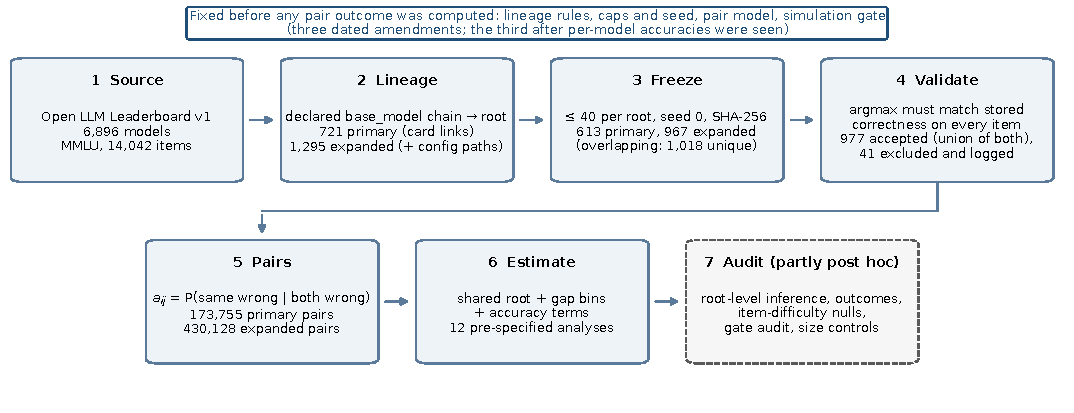
\includegraphics[width=\textwidth]{fig_workflow.pdf}
\caption{\textbf{Study workflow.} Counts are read from the analysis outputs. The primary and expanded samples overlap; 977 is the number of unique accepted models across both. Steps 2--6 were fixed before any pair outcome was computed (three dated amendments, Section~\ref{sec:gate}); step 7 combines pre-registered secondary analyses with exploratory and post-hoc audits. Primary and expanded populations differ only in the lineage evidence accepted (Section~\ref{sec:lineage}); $a_{ij}$ is the outcome of Eq.~\eqref{eq:outcome}.}
\label{fig:workflow}
\end{figure*}

\section{Related Work}
\label{sec:related}

\textbf{Correlated errors in LLMs.} Kim~\textit{et al.}~\cite{kim2025} measure pairwise agreement on wrong answers across 349 Hugging Face models and 71 HELM models and regress it on pair characteristics, finding that a shared provider, a shared base architecture and similar size predict higher agreement, and that larger and more accurate models have more correlated errors even across architectures and providers. They suggest that newer models may be converging in their outputs but do not test this over release time. Chen~\cite{chen2026} shows, across 67 models, that the gain from routing, voting or mixture-of-agents is capped by the rate at which all models fail the same query, and that average pairwise error correlation understates that rate. Kuai~\textit{et al.}~\cite{kuai2026} audit 18 models from six families for synchronized failures with difficulty-weighted dependence metrics, relate dependence to judges over-endorsing responses, and reweight verifier ensembles accordingly. Goel~\textit{et al.}~\cite{goel2025} propose a chance-adjusted similarity metric based on overlapping mistakes and report that mistakes become more similar as capability increases. Our temporal predictor is different from both accuracy-related correlation and model age: it is the \emph{proximity} of two models' release months, estimated at equal lineage status and conditional on both models' accuracies, which the model controls for (the accuracy-sum coefficient is positive, consistent with~\cite{kim2025}). We make no claim about absolute model age.

\textbf{Null models for excess agreement.} Jo, Garg and Raghavan~\cite{jo2026} argue that whether models agree ``more than expected'' depends on two analyst choices: the null model of independence, where accounting for item difficulty leads to very different conclusions from nulls that do not, and the population of models and items compared. They conclude that monoculture is a context-dependent inference rather than an absolute property of models. This bears directly on our study, which uses one benchmark and one leaderboard population. Three estimands are in use: correlated correctness (whether two models fail the same items, e.g.\ the phi coefficient of error indicators, or co-failure in excess of an item-difficulty null); conditional agreement on the wrong option (whether two models that both fail an item choose the same distractor~\cite{kim2025}); and accuracy-adjusted similarity~\cite{goel2025}. Our primary estimand is the second and our secondary the first. More importantly, our quantity of interest is a \emph{contrast}---the difference in agreement between pairs that share a lineage root and pairs that do not, at equal release-month gap---not the \emph{level} of excess agreement that the null-model debate concerns. A null that shifts all pairs' expected agreement equally leaves such a contrast unchanged; a null that differs between related and unrelated pairs does not. Section~\ref{sec:itemnull} therefore re-estimates both outcomes against item-difficulty-aware nulls.

\textbf{Our contribution.} We do not claim to be the first study of correlated errors in language models. To our knowledge, and based on the work reviewed here, this is the first study to examine declared fine-tune ancestry and release-month proximity \emph{jointly} as correlates of conditional same-wrong-option agreement, controlling for both models' accuracies and accounting for the dependence of pairs that share a model or a lineage root. Each element differs from the closest prior work: the outcome is conditional agreement on the wrong option (not the all-fail rate of an ensemble~\cite{chen2026}, judge dependence~\cite{kuai2026} or pipeline measurement error~\cite{messing2026}); lineage is declared fine-tune ancestry resolved to a root checkpoint (not provider or architecture labels~\cite{kim2025}, family membership~\cite{kuai2026} or dataset lineage~\cite{li2026roots}); and release time is the gap between two models' upload months, estimated at equal lineage status.

\textbf{Lineage and ancestry.} Laufer, Oderinwale and Kleinberg~\cite{laufer2025} map the family trees of about 1.86 million Hugging Face models from their declared parents and study how metadata traits---licenses, language support, model cards---are inherited and drift along lineages. Horwitz, Shul and Hoshen~\cite{horwitz2025} recover model trees from model weights alone. Both treat lineage as the object of study; neither measures whether related models make the same errors on benchmark items. PhyloLM~\cite{phylolm2024} reconstructs phylogenies of language models from output similarity; Li~\textit{et al.}~\cite{li2026roots} reconstruct the lineage of post-training \emph{datasets} and show that benchmark contamination can propagate along it. These works infer or exploit lineage of models or data; we take lineage from declarations and ask how much error agreement it accounts for relative to release time.

\textbf{Variance components and dyadic inference.} Crossed variance-component models estimated by restricted maximum likelihood~\cite{patterson1971,harville1977,searle1992} underlie the per-model analysis in Section~\ref{sec:precision}; generalizability theory~\cite{brennan2001} asks the same question of measurement facets, and Messing~\cite{messing2026} shows that ignoring design choices in LLM pipelines (judge model, temperature, prompt) makes evaluation uncertainty, including on MMLU, look smaller than it is. Pairwise outcomes are not independent, because every model appears in many pairs; we use dyadic cluster-robust variance estimators~\cite{fafchamps2007,cameron2011,aronow2015} and a delete-one-root jackknife~\cite{efron1982}.

\textbf{Ensembles and monoculture.} Ensemble gains depend on error diversity~\cite{dietterich2000,breiman2001,kuncheva2003}; algorithmic monoculture arguments~\cite{kleinberg2021,bommasani2022} treat correlated error as an input. Our results bear on which kind of diversity is associated with less shared error, without testing ensembles directly.

\section{Why Per-Model Variance Decomposition Is Not Enough}
\label{sec:precision}

\subsection{Model and Identification}
Let $Y_i$ be a per-model trait (e.g., accuracy), with family $f(i)$ and release quarter $e(i)$:
\begin{equation}
\begin{aligned}
Y_i &= \mu + \alpha_{f(i)} + \beta_{e(i)} + u_i,\\
\alpha &\sim \mathcal{N}(0,\sigma^2_L),\quad \beta \sim \mathcal{N}(0,\sigma^2_E),\quad u \sim \mathcal{N}(0,\sigma^2_U),
\end{aligned}
\label{eq:vc}
\end{equation}
so that $\operatorname{Var}(\mathbf{y}) = \sigma^2_L Z_F Z_F^\top + \sigma^2_E Z_E Z_E^\top + \sigma^2_U I$, with only the intercept as a fixed effect. The variance components are identified when the covariance basis $\{Z_F Z_F^\top, Z_E Z_E^\top, I\}$ is linearly independent. The rank of the fixed-effects dummy design $[\mathbf{1} \mid Z_F \mid Z_E]$, used as the gate in the earlier version of this work, is not the relevant condition for this model: for the sixteen models evaluated there, that design is rank-deficient (rank 14 of 15) while the covariance basis has full rank (3 of 3). Its condition number also depends on the arbitrary choice of reference level (TABLE~\ref{tab:precision}).

\subsection{Precision}
Identification does not imply precision. For each design we compute the expected restricted-likelihood information $I_{jk} = \tfrac12\operatorname{tr}(P V_j P V_k)$ at four share scenarios (lineage-dominant 0.5/0.2/0.3, era-dominant 0.2/0.5/0.3, balanced, and low-signal 0.1/0.1/0.8), the delta-method standard error of each share, and, as the verdict, the Monte Carlo root-mean-square error (RMSE) of the share estimates under the same REML estimator (500 replicates per scenario). The analytic standard error tracks the Monte Carlo RMSE closely (e.g., 0.289 versus 0.285 for the sixteen-model design), so it can be used before any measurement.

\begin{table*}[!t]
\caption{\textbf{Precision of family and era variance shares for per-model traits.} FE: fixed-effects dummy design used as a gate in the earlier version; $\kappa$ range is over every choice of reference levels. Covariance-basis rank 3/3 means the variance components are identified. The last column is the worst-case Monte Carlo RMSE of either share across four scenarios (500 replicates each).}
\label{tab:precision}
\centering
\footnotesize
\begin{tabular}{lcccccc}
\toprule
Design & Families & Quarters & FE full rank & $\kappa(X^\top X)$ range & Cov.\ basis & Worst RMSE \\
\midrule
\tabinput{../tables/tab_precision.tex}
\bottomrule
\end{tabular}
\end{table*}

No design reaches an RMSE of 0.10 for both shares (TABLE~\ref{tab:precision}): not the sixteen evaluated models (0.30), not the 47-model candidate frame (0.19), and not the 30-model configuration the earlier version described as sufficient (0.19). Removing the single model responsible for the fixed-effects rank deficiency leaves the RMSE unchanged (0.302). The binding constraint is the number of \emph{levels} of each factor: more models per level help only up to a point (with six families and fourteen quarters, 22 models give 0.256 and 47 give 0.189). In staggered designs (Fig.~\ref{fig:scaling}), bringing both shares within $\pm 0.10$ requires on the order of sixty families and fourteen quarters; with eight quarters the era share never falls below about 0.14. Because release quarters are few by construction, a per-model decomposition is a poor instrument for RQ2--RQ3 in populations like those examined here. Within the designs and scenarios examined, this answers RQ1 in the negative and motivates the pair-level design; it does not show that the shares are inestimable under every design, only that the required numbers of families and quarters exceed those available.

\begin{figure}[!t]
\centering
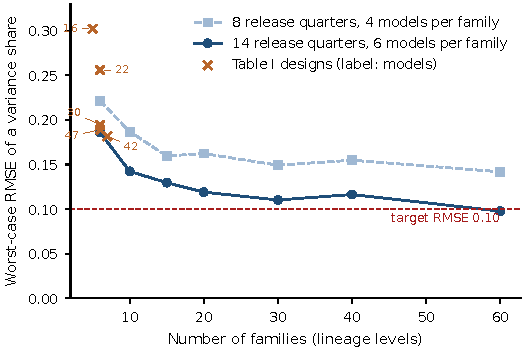
\includegraphics[width=\columnwidth]{precision_scaling.pdf}
\caption{\textbf{Precision of per-model variance shares versus the number of families.} Worst-case Monte Carlo RMSE of the family or era share across four scenarios (300 replicates each) for staggered designs with 8 or 14 release quarters, and for the five candidate designs of TABLE~\ref{tab:precision} (crosses, labelled by number of models; 5--7 families). The RMSE is a Monte Carlo root-mean-square error of the estimated share, not the half-width of a confidence interval. The dashed line marks 0.10; only the largest staggered design with 14 quarters (60 families, 360 models) reaches it.}
\label{fig:scaling}
\end{figure}

\section{Pair-Level Design}
\label{sec:design}

\subsection{Outcome}
For models $i$ and $j$ evaluated on the same $K = 14{,}042$ MMLU items~\cite{hendrycks2021}, let $c_{ik}$ be model $i$'s chosen option on item $k$ (the argmax of its per-option log-likelihoods) and $g_k$ the correct option. The outcome is the conditional agreement~\cite{kim2025}
\begin{equation}
a_{ij} = \frac{\sum_k \mathbf{1}[c_{ik} = c_{jk} \neq g_k]}{\sum_k \mathbf{1}[c_{ik} \neq g_k]\,\mathbf{1}[c_{jk} \neq g_k]},
\label{eq:outcome}
\end{equation}
the probability of choosing the same wrong option given that both are wrong. Every pair contributes all items on which both models are wrong; in the data this denominator ranges from 1{,}166 to 10{,}820 items (median 4{,}109 in the primary sample), so every $a_{ij}$ is estimated from more than a thousand items.

\textbf{What the outcome measures.} Each MMLU item has three wrong options. If two models that both err chose among them independently and uniformly, $a_{ij}$ would be $1/3$; values above $1/3$ arise either because some distractors are more attractive to all models, or because the two models share a preference. The outcome therefore separates two questions that are often merged: \emph{whether} two models fail on the same items (correlated correctness, measured here by the secondary outcome, the phi coefficient of the two error indicators), and \emph{how} they fail when they do (which distractor they choose). Conditioning on joint failure removes most of the mechanical dependence of agreement on accuracy, because two weak models are not counted as agreeing merely for being wrong often; it does not remove all of it, which is why accuracy enters the model below. Because $a_{ij}$ is a ratio over a pair-specific set of items, pairs with low accuracy are evaluated on more, and on average easier, items than pairs with high accuracy; the item-difficulty-aware nulls of Section~\ref{sec:itemnull} address this directly.

\textbf{Estimand.} The quantity of interest is a \emph{contrast} between kinds of pairs, not the level of $a_{ij}$: how much more often two models agree on wrong options when they descend from the same root, at equal release-month gap and equal accuracies, and how much more often they agree when released close together, at equal lineage status and equal accuracies. Fig.~\ref{fig:schematic} illustrates the two predictors. Every pair has one value of each, so the design crosses them: same-root pairs occur at several gaps and same-month pairs occur with and without a shared root. The two terms are separated only to the extent that these combinations are populated, which Section~\ref{sec:lineage} documents.

\begin{figure}[!t]
\centering
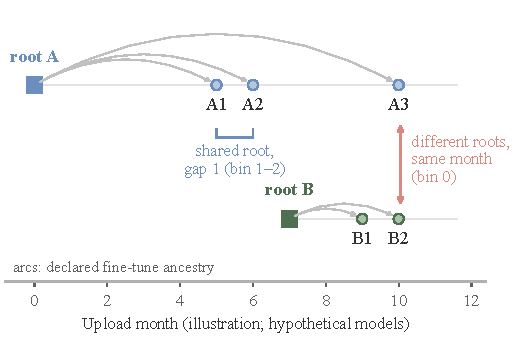
\includegraphics[width=\columnwidth]{fig_schematic.pdf}
\caption{\textbf{The two pair-level predictors} (illustration with hypothetical models). Squares are lineage roots and circles fine-tunes placed at their upload month; arcs show declared ancestry. A1 and A2 share a root and were uploaded one month apart (shared root, gap bin 1--2); A3 and B2 descend from different roots but were uploaded in the same month (no shared root, gap bin 0). Every pair carries one value of each predictor, and the pair model estimates each association at equal levels of the other.}
\label{fig:schematic}
\end{figure}

\subsection{Model and Inference}
\begin{equation}
\begin{aligned}
a_{ij} = {}& b_0 + b_L\, s_{ij} + \textstyle\sum_{g} b_{E,g}\, \mathbf{1}[\,|m_i - m_j| \in g\,]\\
& + c_1 (\mathrm{acc}_i + \mathrm{acc}_j) + c_2 |\mathrm{acc}_i - \mathrm{acc}_j| + \varepsilon_{ij},
\end{aligned}
\label{eq:pair}
\end{equation}
where $s_{ij}$ indicates a shared lineage root, $m_i$ is the model's upload month, and the gap bins are 0, 1--2, 3--5 and 6--11 months with 12 or more as reference. $b_L$ is the association of shared lineage with agreement at equal time gap; $b_{E,0}$ is the association of same-month release at equal lineage status. Both are conditional associations within a pair-level regression, not causal effects of lineage or of release timing. Accuracy terms control for the fact that weaker models have more, and different, errors. Because every model enters many pairs, pair residuals are dependent; the pre-registered standard errors are dyadic cluster-robust~\cite{fafchamps2007,cameron2011,aronow2015}, allowing arbitrary correlation between any two pairs that share a model. With $\mathbf{x}_p$ the covariate vector and $\hat e_p$ the residual of pair $p$, the estimator is
\begin{equation}
\widehat{V}(\hat{\mathbf{b}}) = (X^\top X)^{-1}\Big(\sum_{p,q:\;p \cap q \neq \emptyset} \hat e_p \hat e_q\, \mathbf{x}_p \mathbf{x}_q^\top\Big)(X^\top X)^{-1},
\label{eq:dyadic}
\end{equation}
where $p \cap q \neq \emptyset$ means that pairs $p$ and $q$ share at least one model (including $p = q$). Section~\ref{sec:inference} adds two procedures that treat the lineage root as the unit of dependence: root-level dyadic clustering, Eq.~\eqref{eq:dyadic} with ``share a model'' replaced by ``touch a common root'', and a delete-one-root jackknife, which refits the model $G$ times, each time omitting every pair that involves one of the $G$ roots, and estimates the variance as $\frac{G-1}{G}\sum_g (\hat{\mathbf{b}}_{(g)} - \bar{\mathbf{b}})^2$. Root-level procedures matter because fine-tunes of one root may share errors beyond what their shared membership in pairs captures.

\textbf{Why accuracy is controlled.} Two models of similar accuracy tend to fail on similar items, and the items that strong models fail are the hardest ones, which may have more attractive distractors. Agreement can therefore vary with accuracy for reasons unrelated to lineage or release time. The sum and absolute difference of the two accuracies were pre-registered as controls. They are not neutral: if release time shifts accuracy, part of a release-time relationship runs through accuracy, and the adjusted coefficient describes only the remainder. We therefore also report the unadjusted model (Section~\ref{sec:results}).

\subsection{Simulation Gate and Amendments}
\label{sec:gate}
Before any pair outcome was computed, the design was checked by simulation on the actual roster (roots and months only). For model $i$ with ability $\theta_i \sim \mathcal{N}(0.3, 1)$ and item $k$ with difficulty $d_k \sim \mathcal{N}(0, 1)$, the model answers correctly with probability $\operatorname{logit}^{-1}(\theta_i - d_k)$. If it errs, its wrong option is
\begin{equation}
c_{ik} = \begin{cases}
R_{r(i),k} & \text{with probability } \lambda_L,\\
E_{m(i),k} & \text{with probability } \lambda_E,\\
G_k & \text{with probability } \lambda_G = 0.15,\\
\text{uniform} & \text{otherwise,}
\end{cases}
\label{eq:sim}
\end{equation}
where $R_{r,k}$ is a wrong option preferred by root $r$ on item $k$, $E_{m,k}$ a wrong option preferred in month $m$ (persisting from one month to the next with probability 0.8, so that adjacent months share preferences), and $G_k$ a wrong option preferred by all models. Under this model a lineage effect and a release-time effect act through the same mechanism, a shared preferred distractor, which is the scenario in which the two are hardest to tell apart. The full pair pipeline, Eq.~\eqref{eq:outcome}--\eqref{eq:pair} with dyadic standard errors, was applied to each simulated data set. Three properties were checked: null rejection when $\lambda_L = \lambda_E = 0$; \emph{cross-leakage}, the rate at which the wrong term rejects (the lineage term under a release-time-only truth, or a release-month term under a lineage-only truth), which measures whether the confounding of lineage and time is handled; and power. The pre-registered pass criteria were: null rejection at most 10\%; cross-leakage (the lineage term rejecting under era-only truth, or vice versa) at most 10\%; and power at least 80\% for $\lambda = 0.05$ on both terms. TABLE~\ref{tab:pairgate} shows the gate on the primary roster for three caps on the number of models per lineage root.

\begin{table}[!t]
\caption{\textbf{Pair-level simulation gate (primary roster, 14{,}042 simulated items, 20 replicates per truth).} Null: largest rejection rate under no effect. Leakage: largest cross-term rejection. Power: rejection of the lineage / era term at the stated effect weight.}
\label{tab:pairgate}
\centering
\footnotesize
\begin{tabular}{rrcccc}
\toprule
Cap & $N$ & Null & Leakage & Power $\lambda{=}0.05$ & Power $\lambda{=}0.03$ \\
\midrule
\tabinput{../tables/tab_pairgate.tex}
\bottomrule
\end{tabular}
\end{table}

\textbf{Post-hoc audit of the gate.} With 20 replicates per truth, the rates in TABLE~\ref{tab:pairgate} move in steps of five points. After the results were known, and in response to review, we re-ran the same simulation with 500 replicates per truth (TABLE~\ref{tab:gateaudit} and Fig.~\ref{fig:gateaudit}, Wilson 95\% intervals). This audit does not alter the dated decision above, and we report it against the original criteria. For the chosen design (primary, cap 40), the null rejection rate is 5.8--7.8\% (upper limits up to 10.5\%) and power at $\lambda = 0.05$ is 100\% for both terms, so those criteria are met. Power at $\lambda = 0.03$ is 63\% for lineage and 88\% for release month; the gate did not require power at this effect size. The leakage criterion is \emph{not} met at the strongest era effect: with $\lambda_E = 0.10$ the lineage term rejects in 10.8\% of replicates (95\% CI 8.4--13.8; 12.6\% in the expanded sample), against a threshold of 10\%. Every other leakage rate (era into lineage at $\lambda_E \leq 0.05$, and lineage into either release-month term at all three $\lambda_L$) lies between 3.6 and 7.8\%. The leak is a small positive bias---the lineage estimate rises by $1.4\times 10^{-4}$ (Monte Carlo standard error $0.2\times 10^{-4}$), about 2\% of the simulated era effect---arising because pairs sharing a root were released closer together; applied to the largest observed release-month coefficient ($|b_{E,0}| \leq 0.015$), it implies a bias of about $3\times 10^{-4}$ on a lineage estimate of 0.133. The audit also shows that in the primary design the dyadic standard errors are about 4--6\% smaller than the simulated sampling spread, consistent with null rejection rates slightly above 5\%; in the expanded design they are calibrated. The gate therefore passes its null and power criteria and narrowly fails its leakage criterion at the largest simulated era effect; the root-level inference procedures in Section~\ref{sec:inference}, which give wider intervals, are the appropriate protection. The audit also does not support the 20-replicate choice among caps: the uncapped design (7.2\% leakage) and a cap of 15 (7.2\%) meet all three criteria, and only the chosen cap of 40 narrowly fails; the earlier ranking reflected simulation noise. Cap 40 remains the primary design because it was the dated choice made before any pair outcome was computed; it was neither chosen nor retained for its estimate, and switching designs after seeing results would itself be a departure from the pre-registration. Because the cap-15 sample is a subset of the cap-40 sample under the same seeded ordering, we re-estimated the primary model on it (exploratory; 540 validated models): the shared-root coefficient is $+0.146$ (jackknife SE 0.015) and the same-month coefficient $+0.005$ (SE 0.005). The uncapped design could not be analysed, because only the capped samples were downloaded.

\begin{table*}[!t]
\caption{\textbf{Post-hoc gate audit} (500 replicates per truth; Wilson 95\% intervals, in percent). Null: largest rejection rate of any term under no effect. Leakage: largest cross-term rejection across $\lambda \in \{0.03, 0.05, 0.10\}$. Power: rejection of the lineage (L) or release-month (E) term. Not pre-registered.}
\label{tab:gateaudit}
\centering
\footnotesize
\begin{tabular}{lrrcccccc}
\toprule
Sample & Cap & $N$ & Null & Leakage & L, $\lambda{=}0.05$ & E, $\lambda{=}0.05$ & L, $\lambda{=}0.03$ & E, $\lambda{=}0.03$ \\
\midrule
\tabinput{../tables/tab_gateaudit.tex}
\bottomrule
\end{tabular}
\end{table*}

\begin{figure*}[!t]
\centering
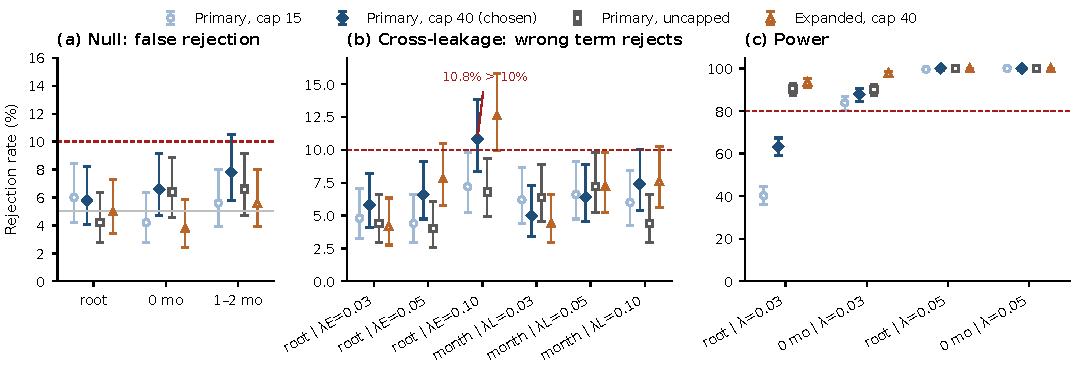
\includegraphics[width=\textwidth]{fig_gate_audit.pdf}
\caption{\textbf{Post-hoc audit of the simulation gate} (500 replicates per truth; bars are Wilson 95\% intervals). (a) Rejection rate of each term when no effect is simulated. (b) Cross-leakage: rejection of the lineage term under release-time-only truths ($\lambda_E$), and of the more often rejecting of the 0- and 1--2-month terms under lineage-only truths ($\lambda_L$). (c) Power of the lineage and same-month terms. Dashed lines mark the pre-registered criteria (10\% for null and leakage, 80\% for power at $\lambda = 0.05$; no power criterion applied at $\lambda = 0.03$). The chosen design (primary, cap 40) exceeds the leakage criterion at $\lambda_E = 0.10$ (10.8\%, interval 8.4--13.8\%), as does the expanded design (12.6\%). Not pre-registered.}
\label{fig:gateaudit}
\end{figure*}

Three amendments were made and dated in the project's pre-registration document, each before the quantities it concerns were computed: (1) the primary data source moved from the second to the first version of the leaderboard, whose item-level files are not access-gated; (2) the per-root cap was set to 40, the only setting meeting all gate criteria (TABLE~\ref{tab:pairgate}), and the gate was re-run with the real item count after an initial run with 1{,}500 items understated power; (3) after the per-model accuracies of the first 443 validated files showed many near-chance models, two sensitivity analyses were added before any pair outcome was computed: S1 adds the total-variation distance $\tfrac12\sum_{o}|\pi_i(o) - \pi_j(o)|$ between the two models' distributions $\pi$ over chosen answer options as a covariate (an answer-option-distribution control: two models that both favor the same letters agree more for that reason alone, whatever their lineage), and S2 restricts to models with accuracy $\geq 0.30$. Amendment 3 is the one decision informed by data: it followed inspection of per-model accuracies, which were needed for validation, but preceded every pair outcome. TABLE~\ref{tab:status} lists the status of every analysis reported, and of two pre-registered secondary analyses that were not carried out.

\begin{table}[!t]
\caption{\textbf{Status of each analysis.} Pre-reg.: in the pre-registration. Amend.: dated amendment made before any pair outcome was computed (Amendment 3 after per-model accuracies were seen). Explor.: not pre-registered, run with or after the pre-registered analyses. Post hoc: added in response to review.}
\label{tab:status}
\centering
\footnotesize
\setlength{\tabcolsep}{3pt}
\begin{tabular}{p{0.63\columnwidth}l}
\toprule
Analysis & Status \\
\midrule
Pair model, Eq.~\eqref{eq:pair}; model-level dyadic SEs & Pre-reg. \\
Phi of error indicators (secondary outcome) & Pre-reg. \\
Simulation gate and its criteria & Pre-reg. \\
Leaderboard version~1 as source & Amend.~1 \\
Primary, expanded and strict populations; cap 40 & Amend.~2 \\
S1 (option distribution), S2 (accuracy $\geq 0.30$) & Amend.~3 \\
\midrule
Root-level dyadic SEs, delete-one-root jackknife & Explor. \\
WLS; $\geq 1{,}000$ jointly wrong items; minus option chance & Explor. \\
Size and architecture controls; root-clustered E1 & Explor. \\
\midrule
500-replicate gate audit; cap-15 subset & Post hoc \\
Raw (no accuracy terms) vs adjusted & Post hoc \\
Item-difficulty-aware nulls N1a, N1b, N2 & Post hoc \\
\midrule
Tree distance as lineage predictor (secondary) & Not done \\
Replication on leaderboard version~2 & Not done$^{a}$ \\
\bottomrule
\end{tabular}

\smallskip
{\footnotesize $^{a}$Version-2 item-level files are access-gated (Amendment~1).}
\end{table}

\section{Data}
\label{sec:data}

\subsection{Source and Validation}
The first version of the Open LLM Leaderboard~\cite{beeching2023} evaluated thousands of open-weight models on MMLU (5-shot) with the LM Evaluation Harness~\cite{gao2021} and published per-item details, including per-option log-likelihoods. For each model we select the most complete run covering all 57 subjects and read four fields per item: the per-option log-likelihoods, the gold option, the leaderboard's stored per-item correctness and, where present, an item hash. We accept the model only if (i) all 14{,}042 items are present, (ii) the argmax of the per-option scores reproduces the stored per-item correctness on \emph{every} item, and (iii) item order and gold answers match a reference model. Three storage layouts occur; in the newest, the gold column is empty and gold is taken from the reference by position, which check (ii) then validates (a misaligned gold vector fails on roughly three quarters of items). Extracted macro-accuracy equals the leaderboard's official results files for the models we spot-checked (43.80, 70.06 and 75.56). For each accepted model we store the chosen option (the argmax), the gold option, the item identifier and hash, the run identifier and the file layout; the per-option scores are used for validation and not retained. Fig.~\ref{fig:validation} shows the procedure and where models were rejected.

Check (ii) is the substantive one. The earlier version of this work failed precisely here: its evaluation code read one field per item and recorded the first answer option for every question, producing constant predictions that no aggregate statistic flagged (Appendix~\ref{app:v1}). Requiring the extracted answer to reproduce the leaderboard's own correctness flag on all 14{,}042 items rules out that failure, a misaligned item order, and a misread gold column, because each of these produces thousands of disagreements. It cannot detect an error in the leaderboard's evaluation itself, such as an unsuitable prompt format for a particular model (Section~\ref{sec:limitations}).

\begin{figure}[!t]
\centering
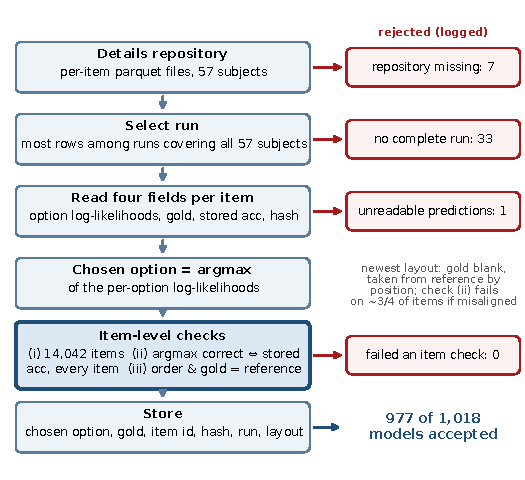
\includegraphics[width=\columnwidth]{fig_validation.pdf}
\caption{\textbf{Prediction extraction and validation} for the 1{,}018 models in the two frozen samples. Rejections are logged with their reason and were not replaced. Check (ii) compares the argmax of the per-option log-likelihoods with the leaderboard's stored per-item correctness on every item; no model that reached this step failed it.}
\label{fig:validation}
\end{figure}

\subsection{Lineage and Release Time}
\label{sec:lineage}
Lineage is resolved by following each model's declared \texttt{base\_model} on Hugging Face to a root, collapsing repository renames and a short, documented list of straight re-uploads and quantisations. A chain is unresolved if it passes through a merge (several parents), reaches a deleted or invalid ancestor, or ends at a fine-tune with no declared parent. Two populations are frozen: \emph{primary}, in which every link comes from a model card, and \emph{expanded}, which additionally accepts a model's own first link from the \texttt{\_name\_or\_path} field of its configuration file when that field names an existing Hugging Face repository (valid for 1{,}066 of 2{,}978 models lacking a card declaration, of which 574 then resolved to an eligible root; local paths, merge-tool paths and self-references were rejected). A \emph{strict} variant keeps only chains ending at a checkpoint the leaderboard lists as pretrained. Release time is the Hub creation month of the model repository (27 distinct months, March 2022 to July 2024).

\subsection{Model Flow}
Fig.~\ref{fig:population} reconciles the populations. The two frozen samples (at most 40 models per root, fixed seed) overlap in 562 models and together comprise 1{,}018; 977 passed validation and 41 were excluded and documented (33 without a complete MMLU run, 7 whose details repository is missing, and 1 with unreadable predictions). No excluded model was replaced. Every exclusion was decided before any pair outcome was computed.

\begin{figure}[!t]
\centering
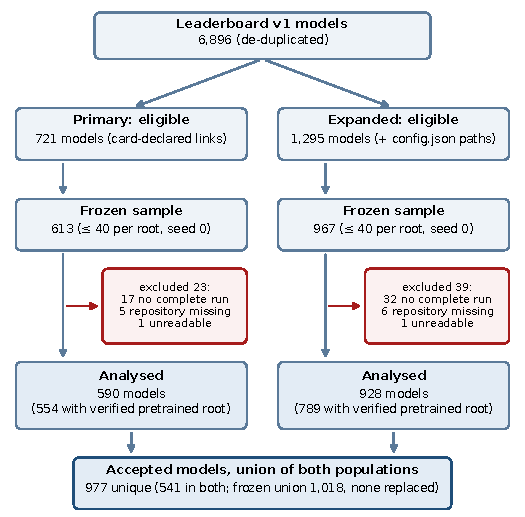
\includegraphics[width=\columnwidth]{fig_population.pdf}
\caption{\textbf{Model populations and exclusions.} The primary population accepts only lineage links declared on model cards; the expanded population also accepts a model's first link from its configuration file. Each frozen sample holds at most 40 models per lineage root (seed 0); exclusions are counted per sample, so models in both samples appear in both columns. ``Verified pretrained root'': the strict variant used in two pre-registered analyses per population.}
\label{fig:population}
\end{figure}

The analysed primary sample comprises 590 models from 351 lineage roots, of which 63 roots contribute two or more models; the expanded sample comprises 928 models from 422 roots (108 with two or more). The largest roots are Llama-3-8B and Mistral-7B-v0.1 (39 and 37 models in the primary sample). Median accuracy is 0.415; 247 of 590 primary models score below 0.30, close to chance for four options, which motivated S1 and S2.

\textbf{How lineage and release time overlap.} Fig.~\ref{fig:lineagemap} places the primary models on a grid of lineage root by upload month. Two features matter for interpretation. First, most roots contribute a single model (288 of 351 in the primary sample); such models enter only different-root pairs, and the lineage contrast is identified by the 63 roots with two or more models. Second, the fine-tunes of a root are uploaded within a few months of one another, and the fine-tunes of the largest roots were uploaded in late 2023 and 2024, so same-root pairs are concentrated at short gaps (711, 1{,}004, 259, 45 and 1 pairs in the 0, 1--2, 3--5, 6--11 and 12+ month bins). Release-month gaps of a year or more are populated almost entirely by different-root pairs. The lineage coefficient is therefore estimated mainly from comparisons at gaps under six months, and the release-time coefficients mainly from different-root pairs; the simulation gate was designed to test whether this structure lets either term absorb the other.

\begin{figure*}[!t]
\centering
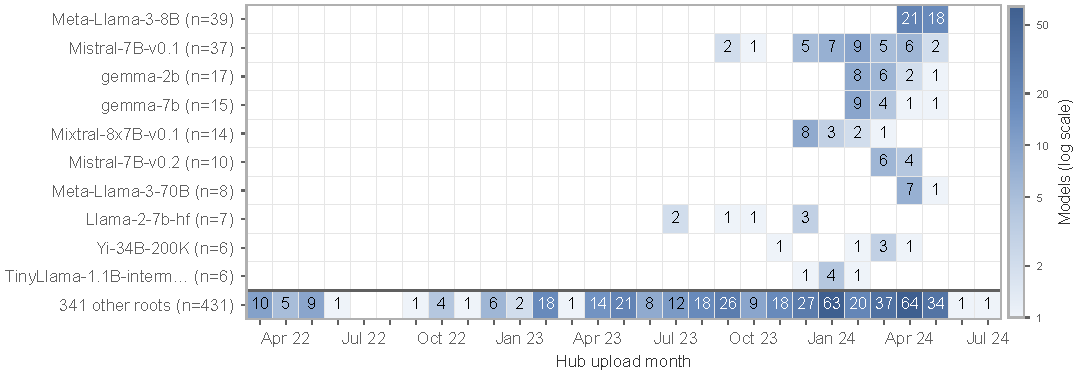
\includegraphics[width=\textwidth]{fig_lineage_month_map.pdf}
\caption{\textbf{Lineage roots by upload month} (primary sample, 590 models). Each cell counts the analysed models of one root uploaded in one month (log color scale; empty cells blank). The 10 largest roots are shown individually; the bottom row pools the remaining 341 roots, most of which contribute a single model. Fine-tunes of a root cluster within a few months, so same-root pairs are concentrated at short release-month gaps.}
\label{fig:lineagemap}
\end{figure*}

\section{Results}
\label{sec:results}

\subsection{Primary Result and Pre-Registered Robustness}
\textbf{Primary result.} In the pre-registered primary analysis (590 models, 173{,}755 pairs), two models that share a lineage root choose the same wrong option, when both are wrong, 13.3 percentage points more often than two models from different roots at the same release-month gap and accuracies (95\% CI 11.8--14.8; delete-one-root jackknife CI 10.8--15.8). Two models released in the same month do so 0.4 points more often than two released a year or more apart, at equal lineage status and accuracies (CI $-0.3$ to $+1.1$). The rest of this section shows that the first estimate is stable across specifications, inference procedures, outcomes and nulls, and that the second is not stable in sign or magnitude.

The mean agreement is 0.423 (primary). Kim~\textit{et al.} report the same mean for their Hugging Face population~\cite{kim2025}, but that population comes from a later leaderboard snapshot with a different question set (12{,}032 questions), so the coincidence is not evidence of validity. Unadjusted, pairs sharing a root agree on 73.1\% of jointly wrong items and other pairs on 42.0\% (Fig.~\ref{fig:gap}). TABLE~\ref{tab:prereg} and Fig.~\ref{fig:forest} report all twelve pre-registered analyses.

\begin{table*}[!t]
\caption{\textbf{Pre-registered analyses.} Coefficients of Eq.~\eqref{eq:pair} with 95\% confidence intervals from dyadic (model-level) cluster-robust standard errors. ``Same month'' is the 0-month gap bin relative to 12 or more months; $p$ refers to it.}
\label{tab:prereg}
\centering
\footnotesize
\begin{tabular}{lrrccc}
\toprule
Analysis & Models & Pairs & Shared root & Same month & $p$ (same month) \\
\midrule
\tabinput{../tables/tab_prereg.tex}
\bottomrule
\end{tabular}
\end{table*}

\begin{figure}[!t]
\centering
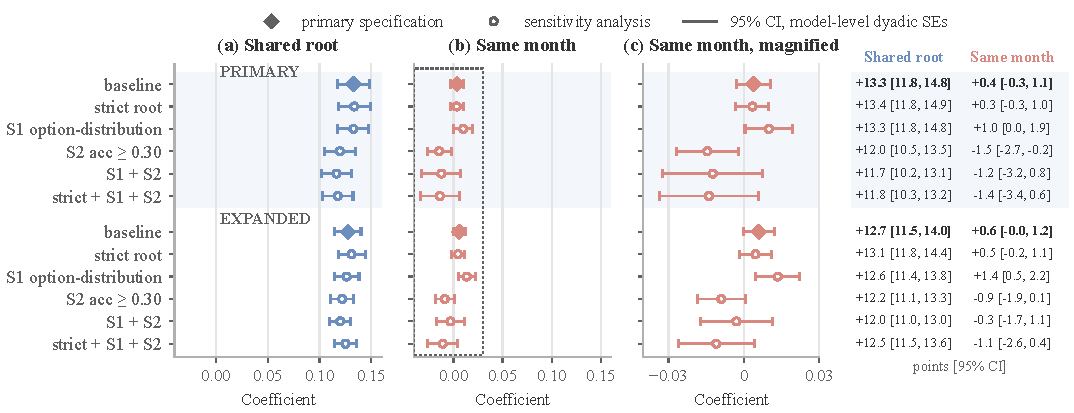
\includegraphics[width=\columnwidth]{exp04_forest.pdf}
\caption{\textbf{Shared-root and same-month coefficients across the twelve pre-registered analyses} (95\% CIs from model-level dyadic cluster-robust standard errors). Diamonds: the primary specification of each population; open circles: the pre-registered sensitivity analyses. Strict: root verified as a pretrained checkpoint. S1: adds the answer-option-distribution covariate. S2: models with accuracy $\geq 0.30$. Note the different horizontal scales: every shared-root interval lies above 0.10, while same-month estimates lie within $\pm 0.02$ and change sign between specifications. Root-level intervals are in Fig.~\ref{fig:inference}.}
\label{fig:forest}
\end{figure}

\begin{figure}[!t]
\centering
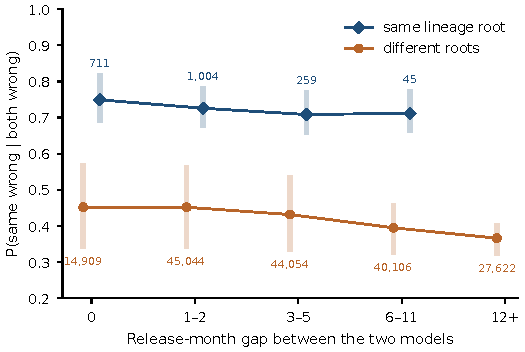
\includegraphics[width=0.8\columnwidth]{exp04_agreement_by_gap.pdf}
\caption{\textbf{Unadjusted agreement on wrong answers by release-month gap} for pairs sharing a lineage root and other pairs (primary sample). Points: mean of $a_{ij}$; shaded bars: interquartile range across pairs; labels: number of pairs. Bins with fewer than 20 pairs are omitted (one same-root pair is 12 or more months apart). The gap between the two lines is present at every release-month gap; the decline of the lower line with gap is the unadjusted release-time gradient, which is not the adjusted association: it is accounted for by accuracy similarity (Fig.~\ref{fig:rawadj}).}
\label{fig:gap}
\end{figure}

Fig.~\ref{fig:gap} shows the raw pattern behind these estimates. At every release-month gap at which both kinds of pair occur, same-root pairs agree on 71--75\% of jointly wrong items and different-root pairs on 40--45\%. Among different-root pairs agreement declines slowly with the gap, from 0.45 in the same month to 0.37 at a year or more.

\textbf{Lineage (RQ2).} In the primary analysis, sharing a root is associated with a 13.3-point higher agreement (95\% CI 11.8--14.8). Across the twelve analyses the estimate ranges from 11.7 to 13.4 points; every confidence interval excludes zero by a wide margin. Controlling for the answer-option distribution (S1) leaves it unchanged; restricting to models above 0.30 accuracy (S2) reduces it slightly, to about 12 points.

\textbf{Release time (RQ3).} In the primary analysis the same-month coefficient is $+0.004$ (CI $-0.003$ to $+0.011$, $p = 0.26$). It is positive and nominally significant when the answer-option distribution is controlled ($+0.010$, CI $+0.0005$ to $+0.0195$, $p = 0.04$), and negative when near-chance models are excluded ($-0.015$, CI $-0.027$ to $-0.002$, $p = 0.02$ in the primary S2 analysis; $-0.009$, $p = 0.07$ in the expanded S2 analysis). The 1--2, 3--5 and 6--11-month bins show the same pattern. Net of accuracy, the release-time association is therefore not stable in sign or magnitude across specifications; where coefficients are nominally significant they are an order of magnitude smaller than the lineage association and change sign between specifications. This is a lack of consistent evidence, not evidence that the association is zero. It is also conditional on accuracy. TABLE~\ref{tab:rawadj} reports the model with and without the pre-registered accuracy terms. Without them, release proximity has a graded association (same month $+0.087$, falling to $+0.029$ at 6--11 months) and the shared-root coefficient is $+0.283$; with them, every release-month coefficient is near zero and the shared-root coefficient is $+0.133$. The unadjusted release-time gradient, and about half of the unadjusted lineage gap, are therefore accounted for by models of similar accuracy agreeing more~\cite{kim2025}. The two columns answer different questions. The adjusted coefficient is the association of release proximity \emph{conditional on} both models' accuracies; because release time can itself shift accuracy, conditioning may remove part of a genuine release-time relationship, and the raw coefficient is the better description of how much more contemporaneous models agree overall. Fig.~\ref{fig:rawadj} shows the comparison for both populations.

\begin{figure}[!t]
\centering
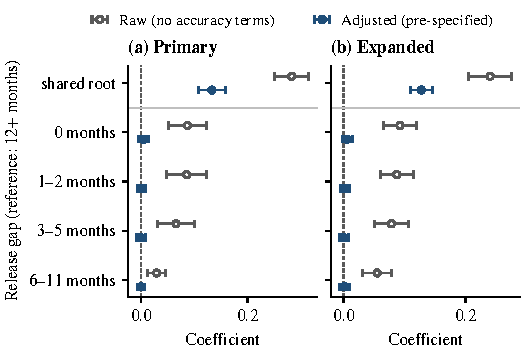
\includegraphics[width=\columnwidth]{fig_raw_adjusted.pdf}
\caption{\textbf{Raw and accuracy-adjusted associations} (delete-one-root jackknife 95\% CIs). Raw: the pre-registered model without the two accuracy terms. Adjusted: the pre-registered model. Release-month bins are relative to the reference category, a gap of 12 or more months. Adding the accuracy terms halves the shared-root coefficient and removes the graded release-time association in both populations. Values: TABLE~\ref{tab:rawadj}.}
\label{fig:rawadj}
\end{figure}

\begin{table*}[!t]
\caption{\textbf{Raw and accuracy-adjusted associations} (primary and expanded samples; 95\% CIs from the delete-one-root jackknife). Raw: Eq.~\eqref{eq:pair} without the accuracy terms. Adjusted: the pre-registered model. Release-month bins are relative to 12 or more months.}
\label{tab:rawadj}
\centering
\footnotesize
\begin{tabular}{lcccc}
\toprule
 & \multicolumn{2}{c}{Primary} & \multicolumn{2}{c}{Expanded} \\
\cmidrule(lr){2-3}\cmidrule(lr){4-5}
Term & Raw & Adjusted & Raw & Adjusted \\
\midrule
\tabinput{../tables/tab_rawadj.tex}
\bottomrule
\end{tabular}
\end{table*}

\subsection{Dependence and Inference}
\label{sec:inference}
The 173{,}755 primary pairs are generated by 590 models, and pairs within a lineage root may be dependent beyond shared membership. TABLE~\ref{tab:inference} compares the pre-registered model-level dyadic standard errors with root-level dyadic clustering, which allows correlation between any two pairs touching the same root, and a delete-one-root jackknife, which removes all pairs involving one root at a time. Root-level procedures widen the interval of the lineage coefficient, by 10--26\% with root-level dyadic clustering and by 39--63\% with the jackknife; its intervals remain far from zero (primary: jackknife CI 10.8--15.8). For the same-month coefficient in the primary S2 analysis, the jackknife interval includes zero ($p = 0.07$), so that negative estimate is not robust to root-level dependence. Fig.~\ref{fig:inference} compares the three procedures. The jackknife gives the widest interval for both terms in all four samples, so it is the conservative reference. Whichever procedure is used, every shared-root interval lies above 0.09, and of the twelve same-month intervals shown only the model-level and root-level dyadic intervals of the primary S2 analysis exclude zero.

\begin{figure}[!t]
\centering
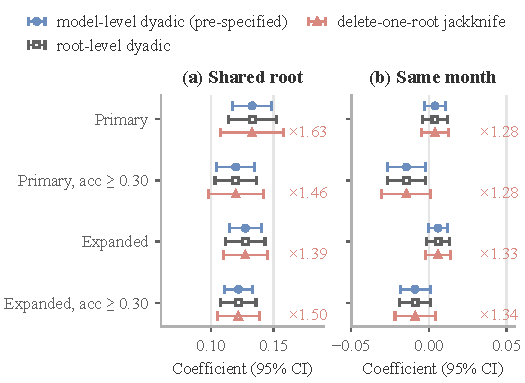
\includegraphics[width=\columnwidth]{fig_inference.pdf}
\caption{\textbf{Sensitivity of the intervals to the unit of dependence.} The pre-registered model-level dyadic intervals allow correlation between pairs sharing a model; root-level dyadic intervals allow it between pairs touching the same lineage root; the jackknife removes one root, and every pair involving it, at a time. Root-level intervals are wider because fine-tunes of one root can err alike in ways not captured by their sharing a model, so the effective number of independent units is closer to the number of roots than of models. Values: TABLE~\ref{tab:inference}.}
\label{fig:inference}
\end{figure}

\begin{table*}[!t]
\caption{\textbf{Inference audit.} $^\dagger$Pre-registered. Root-level procedures treat lineage roots as the unit of dependence.}
\label{tab:inference}
\centering
\footnotesize
\begin{tabular}{lllcc}
\toprule
Sample & Term & Standard error & Estimate [95\% CI] & $p$ \\
\midrule
\tabinput{../tables/tab_inference.tex}
\bottomrule
\end{tabular}
\end{table*}

\subsection{Outcome Definition and Weighting}
TABLE~\ref{tab:outcome} varies the outcome and weighting. Weighting pairs by their number of jointly wrong items raises the lineage estimate slightly (14.2 points) and makes the same-month coefficient positive ($+0.012$, $p = 0.02$). The pre-registered secondary outcome, the phi correlation of error indicators, measures whether two models fail the \emph{same items} rather than choose the same wrong option; it shows a lineage association of $+0.170$ and a smaller, positive same-month association ($+0.018$, CI $+0.010$ to $+0.027$). Subtracting the agreement expected from each model's marginal distribution over answer options (exploratory; an item-level version follows in Section~\ref{sec:itemnull}) leaves the lineage estimate at 12.5 points and the same-month coefficient at $-0.002$. Restricting to pairs with at least 1{,}000 jointly wrong items changes nothing, because every pair already exceeds that threshold. A small, positive association between release proximity and \emph{which items} fail together is therefore plausible; an association with \emph{which wrong option} is chosen is not supported once the answer-option distribution is accounted for. Fig.~\ref{fig:outcomes} shows that the lineage estimate is stable across these definitions, while the same-month estimate is sensitive to both weighting and outcome.

\begin{figure}[!t]
\centering
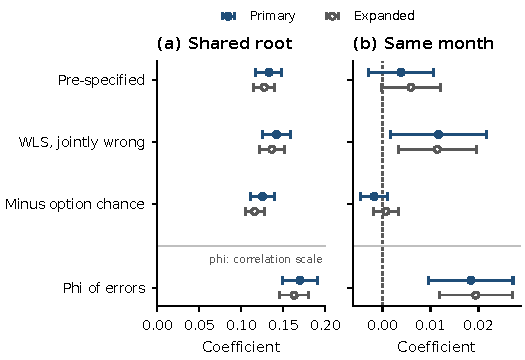
\includegraphics[width=\columnwidth]{fig_outcomes.pdf}
\caption{\textbf{Outcome and weighting variants} (95\% CIs, model-level dyadic). WLS: pairs weighted by the number of jointly wrong items. Minus option chance: agreement minus the agreement expected from the two models' marginal distributions over answer options (exploratory). Phi: the pre-registered secondary outcome, a correlation of error indicators on a different scale. The variant restricted to pairs with at least 1{,}000 jointly wrong items is identical to the pre-registered fit and is omitted. Values: TABLE~\ref{tab:outcome}.}
\label{fig:outcomes}
\end{figure}

\begin{table*}[!t]
\caption{\textbf{Outcome and weighting variants} (dyadic cluster-robust 95\% CIs). Same month: 0-month gap bin relative to 12 or more months.}
\label{tab:outcome}
\centering
\footnotesize
\begin{tabular}{llccc}
\toprule
Sample & Variant & Shared root & Same month & $p$ (same month) \\
\midrule
\tabinput{../tables/tab_outcome.tex}
\bottomrule
\end{tabular}
\end{table*}

\subsection{Item-Difficulty-Aware Nulls}
\label{sec:itemnull}
Added after the results were known, in response to review and following~\cite{jo2026}, these analyses are exploratory. Two nulls condition on the item. \emph{N1} sets the expected agreement on each item to $q_k = \sum_o p_k(o)^2$, where $p_k(o)$ is the share of wrong models choosing wrong option $o$ on item $k$, so that an item with one attractive distractor is expected to produce agreement regardless of lineage; the outcome is observed agreement minus the mean of $q_k$ over the pair's jointly wrong items. N1a computes $p_k$ from all models, which is conservative because a large lineage cluster pulls $p_k$ towards its own choices; N1b weights every lineage root equally. \emph{N2} fits a Rasch model, $\operatorname{logit} P(\text{wrong}_{ik}) = d_k - \theta_i$, by joint maximum likelihood and measures co-failure in excess of $\sum_k \hat{P}_{ik}\hat{P}_{jk}$, per item. TABLE~\ref{tab:itemnull} reports both with delete-one-root jackknife intervals.

Item-level distractor popularity accounts for almost all of the \emph{average} agreement: the mean excess falls from 0.423 to 0.002 (N1a) and 0.019 (N1b), consistent with the observation of~\cite{jo2026} that levels of excess agreement depend on the null. The lineage \emph{contrast} does not change: pairs sharing a root exceed the item-aware expectation by 13.3 points (N1a and N1b, primary), and co-fail on 4.0\% more items than the Rasch model predicts. The same-month coefficient for the choice of wrong option is unchanged ($+0.004$, jackknife $p = 0.37$). For co-failure, a small positive same-month association remains in the full samples ($+0.0036$ per item, jackknife $p = 0.003$) but not among models scoring at least 30\% ($p = 0.56$ and $0.48$). Fig.~\ref{fig:itemnull} shows the central point: the item-level nulls move the \emph{level} of the outcome from 0.42--0.55 to between 0.000 and 0.024, yet the shared-root \emph{contrast} changes by less than 0.002 in every sample. The nulls therefore shift related and unrelated pairs almost equally.

\begin{figure*}[!t]
\centering
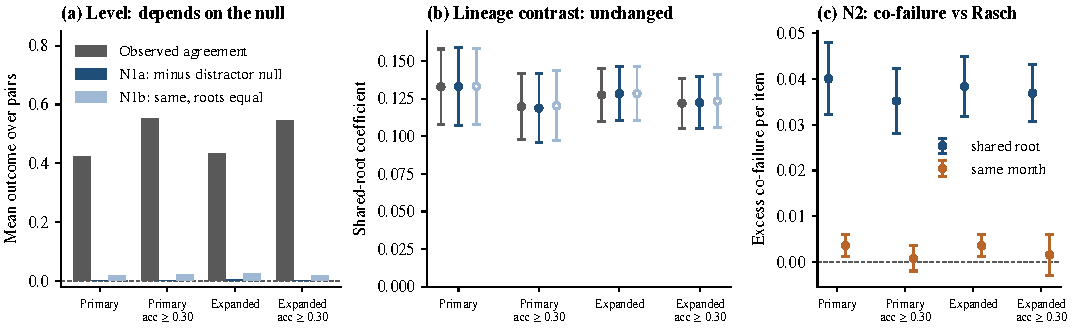
\includegraphics[width=\textwidth]{fig_item_null.pdf}
\caption{\textbf{Item-difficulty-aware nulls} (exploratory, added after review; delete-one-root jackknife 95\% CIs). (a) Mean outcome over pairs: observed agreement on wrong answers, and agreement in excess of the item-level distractor null computed from all models (N1a) or with roots weighted equally (N1b). (b) Shared-root coefficient for the same three outcomes. (c) Excess co-failure over a Rasch null (N2), a measure of whether the same items fail, per item: shared-root and same-month coefficients. Values: TABLE~\ref{tab:itemnull}.}
\label{fig:itemnull}
\end{figure*}

\begin{table*}[!t]
\caption{\textbf{Item-difficulty-aware nulls} (exploratory, added after review). Mean: average outcome across pairs. Estimates with 95\% CIs and $p$-values from the delete-one-root jackknife.}
\label{tab:itemnull}
\centering
\footnotesize
\begin{tabular}{llcccccc}
\toprule
Sample & Outcome & Mean & Shared root & $p$ & Same month & $p$ \\
\midrule
\tabinput{../tables/tab_itemnull.tex}
\bottomrule
\end{tabular}
\end{table*}

\subsection{Exploratory Controls}
Two checks were not pre-registered (TABLE~\ref{tab:exploratory}). Adding model size and same-architecture controls reduces the lineage estimate to 10.2--12.6 points; a shared architecture is associated with a further 0.3--1.8 points. Shared lineage and shared architecture are nested in this population (fine-tunes keep their base architecture), so these coefficients partition one association rather than test two independent ones. Fig.~\ref{fig:controls} shows the comparison. The reduction is largest among models scoring at least 30\%, where a shared architecture also carries its largest coefficient (about 0.018 in both populations); in the full samples the same-architecture coefficient is 0.003--0.005.

\begin{figure}[!t]
\centering
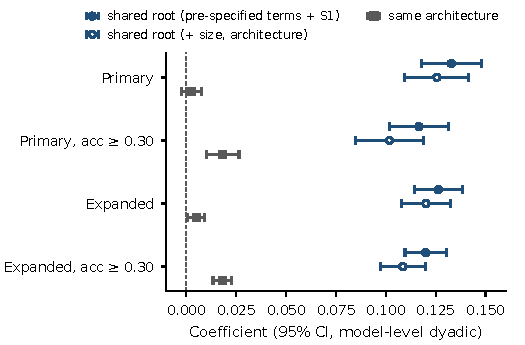
\includegraphics[width=\columnwidth]{fig_controls.pdf}
\caption{\textbf{Size and architecture controls} (exploratory; 95\% CIs from model-level dyadic standard errors). Both models include the pre-registered terms and the S1 covariate; the second adds the absolute difference and sum of log parameter counts and a same-architecture indicator. Values: TABLE~\ref{tab:exploratory}.}
\label{fig:controls}
\end{figure}

\begin{table*}[!t]
\caption{\textbf{Exploratory controls} (not pre-registered; all include the S1 covariate). Entries: estimate (standard error).}
\label{tab:exploratory}
\centering
\footnotesize
\setlength{\tabcolsep}{4pt}
\begin{tabular}{lrcccc}
\toprule
Sample & Models & Shared root (root-clustered SE) & Shared root (+ size, architecture) & Same month (+ size, architecture) & Same architecture \\
\midrule
\tabinput{../tables/tab_exploratory.tex}
\bottomrule
\end{tabular}
\end{table*}

\subsection{Summary of the Evidence}
TABLE~\ref{tab:evidence} collects the findings and the strength of the evidence behind each.

\begin{table*}[!t]
\caption{\textbf{Summary of the evidence.} Estimates refer to the primary sample unless stated; CIs are delete-one-root jackknife intervals.}
\label{tab:evidence}
\centering
\footnotesize
\begin{tabular}{p{0.20\textwidth}p{0.42\textwidth}p{0.30\textwidth}}
\toprule
Question & Finding & Status and caveats \\
\midrule
Shared lineage (RQ2) & $+0.133$ [0.108, 0.158]; 0.117--0.134 across all twelve pre-registered analyses; 0.102--0.142 under root-level inference, alternative weighting, the option-chance-adjusted outcome and size and architecture controls & Pre-registered; observational; identified from 63 roots with two or more models, mostly at gaps under six months \\
Release proximity, adjusted (RQ3) & Same month $+0.004$ [$-0.005$, $+0.013$]; from $-0.015$ to $+0.014$ across the twelve pre-registered analyses, sign not stable & Pre-registered; conditional on both accuracies \\
Release proximity, unadjusted & Same month $+0.087$ [0.051, 0.122], graded with gap; absorbed by the accuracy terms & Post hoc; a total association if accuracy is a mediator \\
Which items fail together & Phi: lineage $+0.170$, same month $+0.018$ (model-level CI 0.010--0.027); excess Rasch co-failure same month $+0.0036$ per item in full samples, not in S2 & Phi pre-registered secondary; Rasch null post hoc \\
Item-level nulls & Average excess agreement 0.002--0.019; lineage contrast unchanged ($\pm 0.002$) & Post hoc \\
Simulation gate & Null and power criteria met; leakage 10.8\% (primary) and 12.6\% (expanded) at $\lambda_E = 0.10$, above 10\%; implied bias on the lineage estimate about $3\times 10^{-4}$ & Post-hoc audit of a pre-registered gate \\
\bottomrule
\end{tabular}
\end{table*}

\section{Discussion}
\label{sec:discussion}

\textbf{What the results say.} Within this population, which open-weight model a fine-tune descends from is strongly associated with which wrong answers it gives: pairs sharing a root agree on wrong answers about 13 points more often, a 31\% increase over the mean. The time at which a model was uploaded adds little, and nothing of consistent sign, to the choice of wrong option. This is consistent with Kim~\textit{et al.}'s finding that a shared provider and architecture predict agreement~\cite{kim2025}, and refines it: with lineage taken from declared ancestry and time measured directly, the association runs through lineage.

\textbf{What they do not say.} The association is observational. Fine-tunes of one base share its parameters, its pretraining data and often similar post-training data; the design does not separate these routes, and it does not show that fine-tuning causes inherited errors. Nor does it show that release time is irrelevant: the pretraining era of a foundation model is a property of its root and therefore nested in lineage here; the release-time estimate is net of accuracy, and contemporaneous models agree more partly because they are similarly accurate; and the phi analysis suggests a small association between release proximity and which items fail together.

\textbf{Adjusted and unadjusted associations.} Without the accuracy terms, models uploaded in the same month agree on wrong answers 8.7 points more often than models uploaded a year or more apart; with them, the difference is 0.4 points. Which number is relevant depends on the role accuracy plays. If release time affects agreement partly \emph{through} accuracy---for example, because models of one period share a level of capability and therefore fail on the same hard items---then accuracy is a mediator, the unadjusted gradient is the total association, and the adjusted coefficient is the part that does not run through accuracy. If instead accuracy and release time are both consequences of something else, such as which base models were available, adjustment removes a confounded component. The data cannot distinguish these readings. What they do show is narrower: once two models' accuracies are known, also knowing how far apart they were released adds nothing of consistent sign about whether they will choose the same distractor, whereas knowing whether they share a root still adds about 13 points. For lineage the choice matters less, because the shared-root coefficient is large under every specification, falling from 28.3 points unadjusted to 13.3 points adjusted.

\textbf{Size of the lineage association.} In raw terms, when two fine-tunes of the same root both fail an item they choose the same distractor about three times in four (73.1\%), against about two times in five (42.0\%) for models from different roots. Net of accuracy and release gap the difference is 13.3 points. The item-difficulty nulls show that this is not an artefact of particular items attracting all models to one distractor: relative to an item-level expectation the excess for same-root pairs is again 13.3 points, while the excess for an average pair is close to zero. Related models are, in this sense, the main source of agreement on wrong answers beyond what the items themselves induce.

\textbf{Why lineage and not release time.} A fine-tune starts from its base model's weights and is typically trained on far less data than its base was pretrained on; it is plausible that much of the base model's knowledge, and its gaps, survive. Models uploaded in the same month, by contrast, share only what was common at the time---popular base models, datasets and recipes---and in this population that commonality is already captured by lineage and by accuracy. These are hypotheses consistent with the results, not mechanisms the design tests.

\textbf{Implications.} For practitioners combining open-weight models, the results suggest a hypothesis: drawing members from different base models may reduce shared wrong-answer behavior more than drawing them from one base at different times. We did not evaluate ensembles, voting or routing, and the effect on ensemble accuracy depends on how members are combined~\cite{chen2026}; whether lineage diversity improves such systems is a question for direct tests.

\section{Limitations and Threats to Validity}
\label{sec:limitations}
\begin{enumerate}
\item \textbf{Population.} The leaderboard population is self-selected and dominated by community fine-tunes of a few dozen bases between 2022 and 2024. Results may not hold for frontier or closed models, or for separately pretrained models released at the same time.
\item \textbf{Era definition.} Release time is the Hub creation month of the fine-tune, not the time its data were collected; pretraining era cannot be separated from lineage in this design.
\item \textbf{Lineage measurement.} Declared \texttt{base\_model} fields can be wrong or missing; models with undeclared lineage are excluded from the primary population, and the expanded population relies on configuration paths that are weaker evidence. A wrong declaration misclassifies pairs: a related pair coded as unrelated, or the reverse. If such errors are unrelated to agreement, they bias the lineage contrast towards zero, so the estimate would be conservative; if models that declare their base carefully also differ systematically in how they err, the bias could go either way. Excluding undeclared models also changes the population, towards fine-tunes with documented ancestry. Estimates agree across the primary (card-declared), expanded (configuration-assisted) and strict (verified-root) populations: 0.127--0.134 in the baseline specifications.
\item \textbf{Conditioning on joint error.} The primary outcome counts only items on which both models are wrong. It describes which wrong option is chosen given joint failure, not the full dependence of two models' errors; the phi outcome covers whether the same items fail, and neither is a direct measure of ensemble performance.
\item \textbf{Benchmark.} One benchmark (MMLU, four options) is used. Many models are near chance; the S1 and S2 analyses and the item-level nulls address this, but preferences over answer options remain a concern for any agreement measure on multiple-choice tests.
\item \textbf{Simulation gate.} The pre-registered gate used 20 replicates per truth. A 500-replicate audit confirms its null and power criteria but finds cross-leakage of 10.8--12.6\% at the largest simulated release-time effect, above the 10\% criterion, and model-level standard errors about 4--6\% too small in the primary design; we therefore report root-level intervals alongside the pre-registered ones.
\item \textbf{Evaluation pipeline.} All predictions were produced by the leaderboard's evaluation pipeline (the LM Evaluation Harness, 5-shot MMLU, log-likelihood scoring), not by us. Model-specific evaluation-configuration errors, including prompt or formatting mismatches, cannot be ruled out and may affect the observed agreement measures. Near-chance accuracy (339 of 977 models below 0.30) does not by itself show a configuration error---many are small or weakly trained models---but it cannot exclude one; the S2 analyses restrict to models above 0.30.
\item \textbf{Null and population dependence.} Following~\cite{jo2026}, levels of excess agreement depend on the null model and on the models and items compared; we report a contrast that is stable across the nulls examined, but other populations or benchmarks may give different contrasts.
\item \textbf{Contamination.} If MMLU items appear in training data, agreement may partly reflect memorization shared by lineage.
\item \textbf{Temporal coverage of lineage pairs.} Pairs sharing a root were almost all released within a year of each other (primary: 711, 1{,}004, 259, 45 and 1 pairs in the 0, 1--2, 3--5, 6--11 and 12+ month bins). The data therefore cannot show whether the lineage association persists between fine-tunes released far apart; an exploratory lineage-by-gap interaction is not identified in the primary sample and is near zero, with wide intervals, in the expanded sample.
\item \textbf{Concentration.} The lineage contrast comes from 63 roots with two or more models in the primary sample (108 expanded), and the two largest roots contribute 39 and 37 models; root-level inference accounts for this dependence, but a few large roots carry substantial weight.
\item \textbf{Post-hoc analyses.} The item-difficulty nulls, the raw-versus-adjusted comparison, the gate audit and the cap-15 subset were added after the results were known (TABLE~\ref{tab:status}); they are reported as checks on the pre-registered estimates, not as independent confirmations.
\item \textbf{Data availability.} The leaderboard's per-item files declare no licence, so the derived answer files are not redistributed and replication requires regenerating them from the public source with the released scripts (Section~\ref{sec:repro}).
\end{enumerate}

\section{Reproducibility}
\label{sec:repro}
{\sloppy
All code, frozen rosters (with SHA-256 hashes), Hub metadata caches, validation reports and analysis outputs are in the project repository at \url{https://github.com/Sudharsanselvaraj/Identifiable-Variance-Decomposition-of-Correlated-Errors-in-Foundation-Models}. A single script (\path{scripts/run_exp04_final.py}) re-runs the twelve pre-registered analyses, the inference and outcome audits and the exploratory checks from the frozen data, verifies the roster hashes, and diffs every coefficient against the committed outputs (maximum absolute difference below $10^{-16}$); all tables in Sections~\ref{sec:design}--\ref{sec:results} are generated from those outputs by \path{scripts/make_exp04_tables.py}, and every figure, including the counts in the two diagrams, by \path{scripts/make_exp04_figures.py}; Fig.~\ref{fig:schematic} is the only illustration with hypothetical models. The leaderboard's per-item details and metadata declare no licence, so neither the derived item-level answer files (103~MB) nor the copied metadata fields are redistributed; the full model lists are rebuilt from the public source by \path{scripts/rebuild_frozen_lists.py}, which verifies them against the SHA-256 hashes recorded when they were frozen, and the answer files are regenerated by \path{scripts/download_ollb_v1.py} from the public leaderboard and validated by \path{scripts/validation_report.py}. The pre-registration and its three dated amendments are in \path{docs/05_Experiments/Exp04_Leaderboard_Lineage_Era.md}.\par}

\section{Conclusion}
\label{sec:conclusion}
Among open-weight models on the first Open LLM Leaderboard, two models that share a declared lineage root choose the same wrong MMLU option, when both are wrong, about 13 percentage points more often than unrelated models at equal release gap and accuracies. The estimate is stable across twelve pre-registered analyses, root-level inference, alternative outcomes and item-difficulty-aware nulls. Net of accuracy, release-month proximity shows no association with the choice of wrong option that is stable in sign or magnitude. The evidence is observational, comes from one benchmark and a population of community fine-tunes, and rests on a design whose simulation gate narrowly missed one of its criteria. The next step is to test whether lineage diversity predicts better ensemble, voting or review performance on other benchmarks, evaluation pipelines and independently pretrained models.

\section*{Acknowledgment}
This work was supported in part by the Department of Computer Science and Engineering, SRM Institute of Science and Technology, Tiruchirappalli, India, and in part by the Research Institute of IoT Cybersecurity, National Kaohsiung University of Science and Technology, Kaohsiung, Taiwan.

\textbf{Use of AI-generated content.} The authors used Claude (Anthropic; model Claude Opus 5.5, accessed through Claude Code)~\cite{claude2026} in October 2026, with substantial use. It wrote and debugged the analysis, simulation, data-extraction and figure/table-generation code, and drafted the text of every section of this revised manuscript (Sections~I--IX and Appendix~A). The authors directed the study, approved each analysis decision and pre-registration amendment, reviewed and edited the text, and take full responsibility for the content; every reported number is produced by the released code from the committed outputs.

\begin{thebibliography}{30}

\bibitem{kim2025} E.~Kim, A.~Garg, K.~Peng, and N.~Garg, ``Correlated errors in
large language models,'' in \emph{Proc. Int. Conf. Mach. Learn. (ICML)},
vol.~267, pp.~30038--30066, 2025.

\bibitem{chen2026} J.~L.~Chen, ``When does combining language models help? A
co-failure ceiling on routing, voting, and mixture-of-agents across 67 frontier
models,'' \emph{arXiv preprint arXiv:2606.27288}, 2026.

\bibitem{goel2025} S.~Goel, J.~Struber, I.~A.~Auzina, K.~K.~Chandra,
P.~Kumaraguru, D.~Kiela, A.~Prabhu, M.~Bethge, and J.~Geiping, ``Great models
think alike and this undermines AI oversight,'' \emph{arXiv preprint
arXiv:2502.04313}, 2025.

\bibitem{laufer2025} B.~Laufer, H.~Oderinwale, and J.~Kleinberg, ``Anatomy of a
machine learning ecosystem: 2 million models on Hugging Face,'' \emph{arXiv
preprint arXiv:2508.06811}, 2025.

\bibitem{horwitz2025} E.~Horwitz, A.~Shul, and Y.~Hoshen, ``Unsupervised model
tree heritage recovery,'' in \emph{Proc. Int. Conf. Learn. Represent. (ICLR)},
2025.

\bibitem{phylolm2024} N.~Yax, P.-Y.~Oudeyer, and S.~Palminteri, ``PhyloLM:
Inferring the phylogeny of large language models,'' in \emph{Proc. Int. Conf.
Learn. Represent. (ICLR)}, 2025.

\bibitem{li2026roots} Y.~Li \emph{et al.}, ``Tracing the roots: A multi-agent
framework for uncovering data lineage in post-training LLMs,'' in \emph{Proc.
64th Annu. Meeting Assoc. Comput. Linguist. (Volume 1: Long Papers)}, 2026,
pp.~9606--9625.

\bibitem{kuai2026} C.~Kuai \emph{et al.}, ``A statistical framework for auditing
behavioral dependence and induced bias in LLM judges,'' \emph{arXiv preprint
arXiv:2604.07650v2}, 2026.

\bibitem{patterson1971} H.~D.~Patterson and R.~Thompson, ``Recovery of
inter-block information when block sizes are unequal,'' \emph{Biometrika},
vol.~58, no.~3, pp.~545--554, 1971.

\bibitem{harville1977} D.~A.~Harville, ``Maximum likelihood approaches to variance
component estimation and to related problems,'' \emph{J. Amer. Statist. Assoc.},
vol.~72, no.~358, pp.~320--338, 1977.

\bibitem{searle1992} S.~R.~Searle, G.~Casella, and C.~E.~McCulloch,
\emph{Variance Components}. New York, NY, USA: Wiley, 1992.

\bibitem{brennan2001} R.~L.~Brennan, \emph{Generalizability Theory}. New York, NY,
USA: Springer, 2001.

\bibitem{messing2026} S.~Messing, ``Hidden measurement error in LLM pipelines
distorts annotation, evaluation, and benchmarking,'' \emph{arXiv preprint
arXiv:2604.11581}, 2026.

\bibitem{fafchamps2007} M.~Fafchamps and F.~Gubert, ``The formation of risk
sharing networks,'' \emph{J. Develop. Econ.}, vol.~83, no.~2, pp.~326--350, 2007.

\bibitem{cameron2011} A.~C.~Cameron, J.~B.~Gelbach, and D.~L.~Miller, ``Robust
inference with multiway clustering,'' \emph{J. Bus. Econ. Statist.}, vol.~29,
no.~2, pp.~238--249, 2011.

\bibitem{aronow2015} P.~M.~Aronow, C.~Samii, and V.~A.~Assenova,
``Cluster-robust variance estimation for dyadic data,'' \emph{Political Anal.},
vol.~23, no.~4, pp.~564--577, 2015.

\bibitem{efron1982} B.~Efron, \emph{The Jackknife, the Bootstrap and Other
Resampling Plans}. Philadelphia, PA, USA: SIAM, 1982.

\bibitem{dietterich2000} T.~G.~Dietterich, ``Ensemble methods in machine
learning,'' in \emph{Proc. Int. Workshop Multiple Classifier Syst.}, LNCS 1857,
2000, pp.~1--15.

\bibitem{breiman2001} L.~Breiman, ``Random forests,'' \emph{Mach. Learn.},
vol.~45, no.~1, pp.~5--32, 2001.

\bibitem{kuncheva2003} L.~I.~Kuncheva and C.~J.~Whitaker, ``Measures of
diversity in classifier ensembles and their relationship with the ensemble
accuracy,'' \emph{Mach. Learn.}, vol.~51, no.~2, pp.~181--207, 2003.

\bibitem{kleinberg2021} J.~Kleinberg and M.~Raghavan, ``Algorithmic monoculture
and social welfare,'' \emph{Proc. Nat. Acad. Sci. USA}, vol.~118, no.~22,
2021.

\bibitem{bommasani2022} R.~Bommasani, K.~A.~Creel, A.~Kumar, D.~Jurafsky, and
P.~Liang, ``Picking on the same person: Does algorithmic monoculture lead to
outcome homogenization?'' in \emph{Adv. Neural Inf. Process. Syst. (NeurIPS)},
vol.~35, 2022.

\bibitem{jo2026} N.~Jo, N.~Garg, and M.~Raghavan, ``The subjectivity of
monoculture,'' \emph{arXiv preprint arXiv:2602.24086}, 2026.

\bibitem{hendrycks2021} D.~Hendrycks \emph{et al.}, ``Measuring massive multitask
language understanding,'' in \emph{Proc. Int. Conf. Learn. Represent. (ICLR)},
2021.

\bibitem{beeching2023} E.~Beeching \emph{et al.}, ``Open LLM Leaderboard
(2023--2024),'' Hugging Face, 2023. [Online]. Available:
\url{https://huggingface.co/spaces/open-llm-leaderboard-old/open_llm_leaderboard}

\bibitem{claude2026} Anthropic, ``Claude (Claude Opus 5.5), accessed through
Claude Code,'' large language model, Oct. 2026. [Online]. Available:
\url{https://www.anthropic.com/claude}

\bibitem{gao2021} L.~Gao \emph{et al.}, ``A framework for few-shot language model
evaluation,'' Zenodo, 2021, doi: 10.5281/zenodo.5371628.

\end{thebibliography}

\appendices

\section{Changes From the Earlier Version}
\label{app:v1}
The earlier version of this manuscript (archived in the repository as \texttt{paper/src/archive/}) reported a sixteen-model evaluation and an identifiability gate. TABLE~\ref{tab:v1} lists each finding of that version that is withdrawn or corrected, why, and how it is treated here.

\begin{table}[H]
\caption{\textbf{Findings of the earlier version and their treatment.}}
\label{tab:v1}
\centering
\scriptsize
\setlength{\tabcolsep}{2.5pt}
\begin{tabular}{p{0.31\columnwidth}p{0.36\columnwidth}p{0.27\columnwidth}}
\toprule
Earlier claim & Reason & Current treatment \\
\midrule
Variance components ``not identifiable'' (fixed-effects dummy-design gate) & Random-effects model identified (basis rank 3/3); condition number depends on reference level (115--585) & Withdrawn; imprecision quantified (Section~\ref{sec:precision}) \\
Item-level predictions; Qwen-7B accuracy 0.2294 & Code read only option~A's log-likelihood; 0.2294 is the all-A rate & Withdrawn; code fixed; validation against stored correctness (Section~\ref{sec:data}) \\
30-model design ``passes'' at $\kappa \leq 50$ & Its $\kappa$ is 93 & Corrected \\
Sweep enforced crossing and connectedness & 100 of 105 crossed, 60 connected & Corrected \\
LPM and GLMM both hit the era boundary in 20--60\% of replicates & Only the GLMM; LPM 0--6.7\% & Corrected \\
Nested-design detector: ``zero silent coverage'' & Undefined: no replicate went undetected & Corrected \\
Sixteen-model population as pre-registered & Four planned models not evaluated, no recorded reason; two DeepSeek models imputed & Arm not used for inference \\
\bottomrule
\end{tabular}
\end{table}


\begin{IEEEbiographynophoto}{Sudharsan S}
is currently pursuing the B.Tech. degree in Computer Science and Engineering at the SRM Institute of Science and Technology, Tiruchirappalli, India. His research interests include natural language processing, large language model evaluation, and variance decomposition methods.
\end{IEEEbiographynophoto}

\begin{IEEEbiographynophoto}{S. Kanaga Suba Raja}
received the B.E. and M.E. degrees in Computer Science and Engineering. He is currently an Assistant Professor with the Department of Computer Science and Engineering, SRM Institute of Science and Technology, Tiruchirappalli, India, and a Visiting Researcher with the Research Institute of IoT Cybersecurity, National Kaohsiung University of Science and Technology, Kaohsiung, Taiwan. His research interests include machine learning, natural language processing, and statistical methods for AI evaluation.
\end{IEEEbiographynophoto}

\begin{IEEEbiographynophoto}{Shree Harish V}
received the degree from the SRM Institute of Science and Technology, Tiruchirappalli, India. He is currently with the Department of Computer Science and Engineering (Big Data Analytics), SRM Institute of Science and Technology, Tiruchirappalli, India. His research interests include cybersecurity, IoT, and AI systems.
\end{IEEEbiographynophoto}

\begin{IEEEbiographynophoto}{Chin-Shiuh Shieh}
received the Ph.D. degree in Electrical Engineering. He is currently with the Research Institute of IoT Cybersecurity, Department of Electrical Engineering, National Kaohsiung University of Science and Technology, Kaohsiung, Taiwan. His research interests include wireless networks, cybersecurity, and IoT systems.
\end{IEEEbiographynophoto}

\begin{IEEEbiographynophoto}{Mong-Fong Horng}
received the Ph.D. degree in Electrical Engineering. He is currently with the Research Institute of IoT Cybersecurity, Department of Electrical Engineering, National Kaohsiung University of Science and Technology, Kaohsiung, Taiwan. His research interests include computer networks, cybersecurity, and AI applications.
\end{IEEEbiographynophoto}

\begin{IEEEbiographynophoto}{Lavanya R}
received the degree from the SRM Institute of Science and Technology, Tiruchirappalli, India. She is currently with the Department of Computer Science and Engineering, SRM Institute of Science and Technology, Tiruchirappalli, India. Her research interests include machine learning, data analytics, and AI systems.
\end{IEEEbiographynophoto}



\EOD

\end{document}
